\documentclass[a4paper]{article}
\usepackage[utf8]{inputenc}
\usepackage{amsmath}
\usepackage{amssymb}
\usepackage{mathtools}
\usepackage{amsfonts}
\usepackage{lastpage}
\usepackage{tikz}
\usepackage{float}
\usepackage{textcomp}
\usetikzlibrary{patterns}
\usepackage{pdfpages}
\usepackage{gauss}
\usepackage{fancyvrb}
\usepackage[table]{colortbl}
\usepackage{fancyhdr}
\usepackage{graphicx}
\usepackage[margin=2.5 cm]{geometry}

\definecolor{listinggray}{gray}{0.9}
\usepackage{listings}
\lstset{
	language=,
	literate=
		{æ}{{\ae}}1
		{ø}{{\o}}1
		{å}{{\aa}}1
		{Æ}{{\AE}}1
		{Ø}{{\O}}1
		{Å}{{\AA}}1,
	backgroundcolor=\color{listinggray},
	tabsize=3,
	rulecolor=,
	basicstyle=\scriptsize,
	upquote=true,
	aboveskip={0.2\baselineskip},
	columns=fixed,
	showstringspaces=false,
	extendedchars=true,
	breaklines=true,
	prebreak =\raisebox{0ex}[0ex][0ex]{\ensuremath{\hookleftarrow}},
	frame=single,
	showtabs=false,
	showspaces=false,
	showlines=true,
	showstringspaces=false,
	identifierstyle=\ttfamily,
	keywordstyle=\color[rgb]{0,0,1},
	commentstyle=\color[rgb]{0.133,0.545,0.133},
	stringstyle=\color[rgb]{0.627,0.126,0.941},
  moredelim=**[is][\color{blue}]{@}{@},
}

\lstdefinestyle{base}{
  emptylines=1,
  breaklines=true,
  basicstyle=\ttfamily\color{black},
}

\pagestyle{fancy}
\def\checkmark{\tikz\fill[scale=0.4](0,.35) -- (.25,0) -- (1,.7) -- (.25,.15) -- cycle;} 
\newcommand*\circled[1]{\tikz[baseline=(char.base)]{
            \node[shape=circle,draw,inner sep=2pt] (char) {#1};}}
\newcommand*\squared[1]{%
  \tikz[baseline=(R.base)]\node[draw,rectangle,inner sep=0.5pt](R) {#1};\!}
\cfoot{Page \thepage\ of \pageref{LastPage}}
\DeclareGraphicsExtensions{.pdf,.png,.jpg}
\author{Nikolaj Dybdahl Rathcke (rfq695)}
\title{Sixth Home Assignment \\ Data Analysis}
\lhead{Nikolaj Dybdahl Rathcke (rfq695)}
\chead{Data Analysis}
\rhead{Assignment 6}

\begin{document}
\maketitle
\section*{Question 1}
\subsection*{(1)}
Given an angle $\alpha$ and a vector $w$, we can calculate $\| w \|$. When we make a triangle as in the assignment text, we can calculate $\|p\|$ with law of sines, since we know one angle is $90$ and we know the angle, $\beta$, opposite of $p$ is $180-90-\alpha$. The law of sines, in our example, say that
\begin{align*}
\frac{\| w\|}{sin(\pi/2)}&=\frac{\| p\|}{sin(\beta)} &\Leftrightarrow\\
\| p\|&=sin(\beta)\frac{\|w\|}{sin(\pi/2)} \\
&=sin(\beta)\|w\|
\end{align*}
This is the length of $p$, to find the vector $p$, we need to make it the same ratio as the vector $u$, this is done by multiplying $\frac{u}{\|u\|}$, thus we get
\begin{align}
p&=sin(\beta)\|w\|\frac{u}{\|u\|}
\label{1}
\end{align}
which is the vector $p$ and the projection of $w$ on $u$.

\subsection*{(2)}
The projection vector $p$ is then given by
\begin{align*}
p&=sin(\beta)\|w\|u
\end{align*}
as the denominator in equation (\ref{1}) is just $1$.

\subsection*{(3)}
The length, as we found in (1) of $p$ is given by 
\begin{align*}
sin(\beta)\|w\|
\end{align*}
where $\beta$ is the last unknown angle (which can easily be found) and $\|w\|$ is the length of the given vector $w$.

\newpage
\section*{Question 3}
Consider the following figure where $E_{out}(g)$ is based on the hypothesis $g$ from all datapoints in it. The inner circle is where $E_{out}(g^-)$ is based on hypothesis $g^-$ from the datapoint in that circle. 
\begin{center}
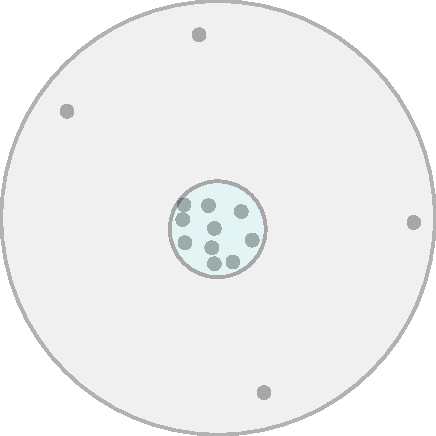
\includegraphics{drawing.pdf}
\end{center}
The out of sample error for on $g$ will be larger as there are outliers, while the error on $g^-$ is less since there are no outliers.

\newpage
\section*{Question 4}
\subsection*{(1)}
The VC-dimension is $27^d$ as $\mathcal{H}_d$ is a tree with depth $d$ and branches $27$ times at every node. Therefore the VC-dimension is $27^d$.


\subsection*{(2)}
The VC-dimension is $\infty$, since the tree has infinite depth.


\subsection*{(3)}
We use corralary (1) from the slides on Occam's razor bound, that states
\begin{align*}
\mathbb{P}\left\{\exists h\in \mathcal{H} : E_{out}-E_{in}> \sqrt{\frac{\ln(M/\delta)}{2N}}\right\}\leq \delta
\end{align*}
We can use this as $\mathcal{H}_d$ is finite, so we replace $M$ by the size and we get the following bound
\begin{align*}
\mathbb{P}\left\{\exists h\in \mathcal{H} : E_{out}-E_{in}> \sqrt{\frac{\ln(27^d/\delta)}{2N}}\right\}\leq \delta
\end{align*}
This is the bound on $E_{out}-E_{in}$ for learning with $\mathcal{H}_d$.

\subsection*{(4)}
From theorem (2) in the slides, we can insert our VC dimension on $H_{d}$ to get
\begin{align*}
\mathbb{P}\left\{\exists h\in \mathcal{H} : E_{out}-E_{in}> \sqrt{\frac{\ln\left(2^{27^d}2^{d+1}/\delta\right)}{2N}}\right\}\leq \delta
\end{align*}

\subsection*{(5)}
The idea of Occam's razor bound is to give each hypothesis a probability. This probability is given by $p(h)$ where $\sum_{h\in \mathcal{H}}p(h)\leq 1$ and as such, the ``burden'' is shared by all hypotheses with a specific weight.

\newpage
\section*{Question 6}
This question is exercise 5.4 in [LFD].
\subsection*{(1)}
The problem with the bound is that it has been invalidated since the learning model has been chosen after the data is observed. So the choice has been based on observations of the data which \textit{likely} fits some learning method instead of figuring our what learning method \textit{should} be used on the dataset. This means we can not know if the bounds are correct.

\subsection*{(2)}
No, as the VC dimension is the outcome of one learning method, that is not nessecarily the right one.

\end{document}